\subsection{Elementy sześcienne}
\label{cha:elementy szescienne}

Obliczenia dotyczące elementów sześciennych zawarte są w modułach katalogu hexahedralElements. Poniżej znajdują się funkcje poszczególnych modułów, wraz z opisem ich zastosowania, argumentami wejściowymi oraz wyjściowymi.

 \( \textbf{Moduł mesh8} \).

\vspace {3mm}
\textit{circleMeshFull(radius, firstCircle, addNodes, circles)} - funkcja działa jak funcja z modułu mesh4 z tą różnicą, że przyjmuje dodatkowy argument addNodes. Określa on ile punktów więcej ma być na każdym kolejnym okręgu siatki.

\vspace {3mm}
\textit{circleMeshSparse(radius, firstCircle, circles)} - funkcja działa jak odpowiednik z modułu mesh4

\vspace {3mm}
\textit{createFiniteElements(vertices, pointsOnLastCircle, length, numberOfPlanes)} - funkcja przyjmuje jako argumenty macierz współrzędnych węzłów, liczbę punktów na ostatnim okręgu siatki, długość modelu pręta oraz liczbę płaszczyzn siatki. Tworzy elementy sześcienne w kilku etapach. Najpierw jedna z płaszczyzn dzielona jest na trójkąty. Następnie trójkąty są łączone w pary i w ten sposób powstają czworokąty. W większości konfiguracji siatki na brzegach pozostają puste miejsca z trójkątów, które nie mają pary. W takich miejscach dodawany jest dodatkowy punkt siatki i z trójkąta tworzony czworokąt. Następnie identyczne czworokąty są tworzone na kolejnych płaszczyznach i wzdłuż długości pręta tworzone są z nich sześciościany. Zwraca macierz e x 8, gdzie e to liczba elementów skończonych. W kolumnach są indeksy kolejnych punktów siatki.

\vspace {3mm}
\textit{brickMesh(radius, numberOfPlanes, numberOfCircles, numberOfPointsOnCircle)} - funkcja tworzy siatkę o kształcie wielokąta na pierwszym okręgu. Przyjmuje jako argumenty promień - radius, liczbę płaszczyzn siatki - numberOfPlanes, liczbę okręgów na płaszczyźnie siatki - numberOfCircles oraz ilość wierzchołków wielokąta wpisanego w okrąg - numberOfPointsOnCircle. Zwraca tablicę o wymiarach n x 3, gdzie n to liczba węzłów. W kolumnach są kolejne współrzędne węzłów.

\vspace {3mm}
\textit{createBrickElements(brickVertices, numberOfPlanes, numberOfCircles, numberOfPointsOnCircle)} - funkcja przyjmuje macierz współrzędnych węzłów z funkcji \textit{brickMesh} - brickVertices, liczbę płaszczyzn siatki - numberOfPlanes, liczbę okręgów na każdej płaszczyźnie - numberOfCircles oraz liczbę wierzchołków wielokąta wpisanego w każdy okrąg - numberOfPointsOnCircle. Tworzy elementy sześciościenne na zadanej siatce. Zwraca macierz e x 8, gdzie e to liczba elementów skończonych. W kolumnach są indeksy kolejnych punktów siatki.

\vspace {3mm}
\textit{drawPlane(vertices)} - jak w mesh4. Przykładowe siatki z tego modułu są przedstawione na rysunku \ref{fig:hex_siatka}.

\vspace {3mm}
\textit{drawBar(vertices)} - jak w mesh4

\vspace {3mm}
\textit{drawTetragons(vertices, indices)} - funkcja przyjmuje jako argumenty macierz współrzędnych węzłów - vertices oraz macierz indeksów węzłów dla każdego elementu - indices. Rysuje układ czworokątów na płaszczyźnie. Przykłady są przedstawione na rysunku \ref{fig:hex_czworokaty}.

\vspace {3mm}
\textit{drawHexahedrons(vertices, indices)} - funkcja przyjmuje jako argumenty macierz współrzędnych węzłów - vertices oraz macierz indeksów węzłów dla każdego elementu - indices. Rysuje model złożony z sześciościanów w rzucie izometrycznym. Przykład znajduje się na rysunku \ref{fig:hex_elementy}.

\begin{figure}
\begin{subfigure}{.5\textwidth}
  \centering
  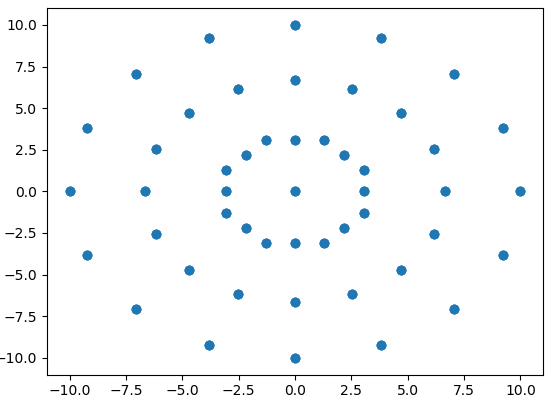
\includegraphics[width=1.0\linewidth]{Zdjecia/5/hex_siatka1}
  \caption{}
  \label{fig:sfig1}
\end{subfigure}
\begin{subfigure}{.5\textwidth}
  \centering
  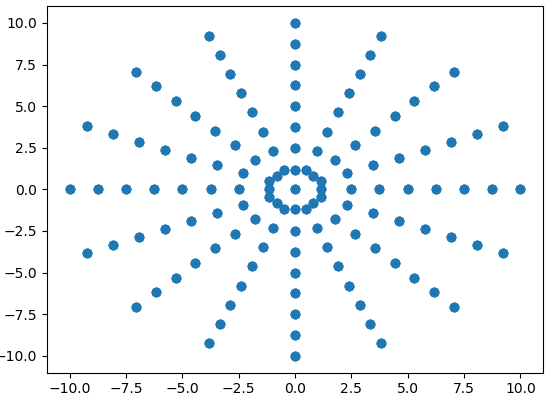
\includegraphics[width=1.0\linewidth]{Zdjecia/5/hex_siatka2}
  \caption{}
  \label{fig:sfig2}
\end{subfigure}
\caption{Układ siatki węzłów na płaszczyźnie powstałych z a) \textit{brickMesh(10, 3, 3, 16)} b) \textit{brickMesh(10, 3, 8, 16)} }
\label{fig:hex_siatka}
\end{figure}

\begin{figure}
\begin{subfigure}{.5\textwidth}
  \centering
  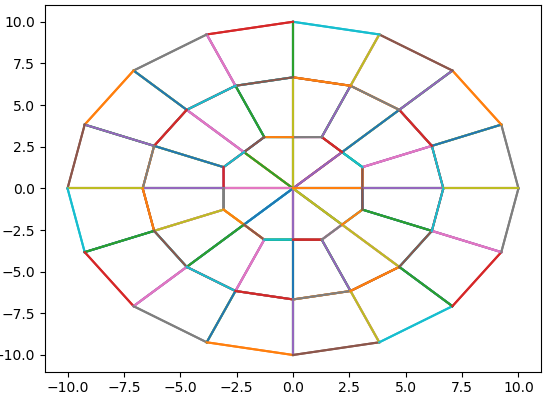
\includegraphics[width=1.0\linewidth]{Zdjecia/5/hex_czworokaty1}
  \caption{}
  \label{fig:sfig1}
\end{subfigure}
\begin{subfigure}{.5\textwidth}
  \centering
  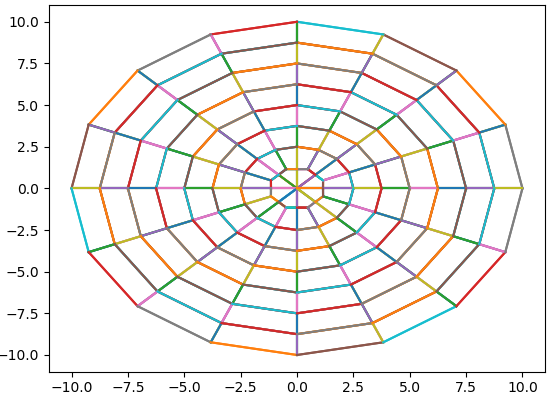
\includegraphics[width=1.0\linewidth]{Zdjecia/5/hex_czworokaty2}
  \caption{}
  \label{fig:sfig2}
\end{subfigure}
\caption{Czworokąty będące ścianą elementu skończonego na płaszczyźnie a) \textit{brickMesh(10, 3, 3, 16)} b) \textit{brickMesh(10, 3, 8, 16)} }
\label{fig:hex_czworokaty}
\end{figure}

\begin{figure}
\begin{subfigure}{.5\textwidth}
  \centering
  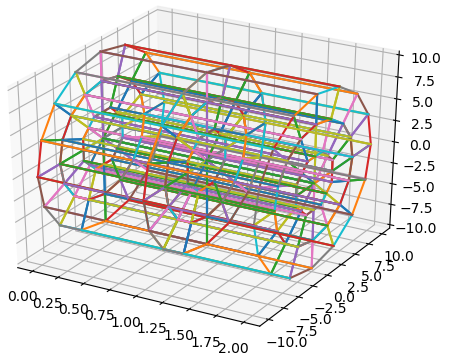
\includegraphics[width=1.0\linewidth]{Zdjecia/5/hex_elementy1}
  \caption{}
  \label{fig:sfig1}
\end{subfigure}
\begin{subfigure}{.5\textwidth}
  \centering
  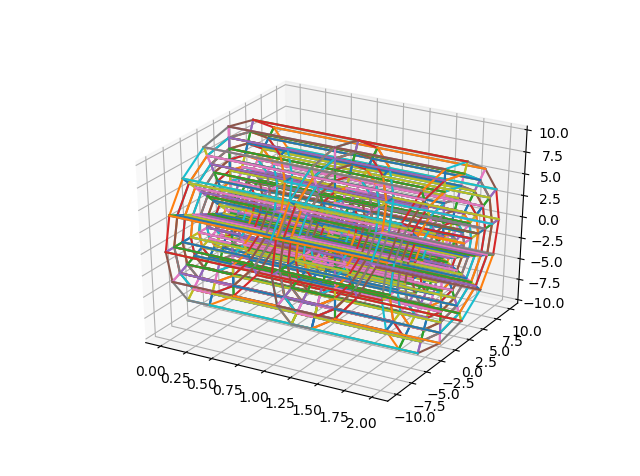
\includegraphics[width=1.0\linewidth]{Zdjecia/5/hex_elementy2}
  \caption{}
  \label{fig:sfig2}
\end{subfigure}
\caption{Elementy skończone zbudowane na siatce a) \textit{brickMesh(10, 3, 3, 16)} b) \textit{brickMesh(10, 3, 8, 16)} }
\label{fig:hex_elementy}
\end{figure}

\vspace {3mm}
 \( \textbf{Moduł calculations8} \).

\vspace {3mm}
\textit{localStiffMatrix(elementVertices)} - funkcja przyjmuje jako argumenty macierz współrzędnych węzłów elementu skończonego. Zwraca macierz sztywności elementu skończonego.

\vspace {3mm}
\textit{localMassMatrix(elementVertices)} - funkcja przyjmuje jako argumenty macierz współrzędnych węzłów elementu skończonego - elementVertices. Zwraca macierz mas elementu skończonego.

\vspace {3mm}
 \( \textbf{Moduł assembling8} \).

\vspace {3mm}
\textit{assembleGlobalStiffMatrix(vertices, indices)} - funkcja przyjmuje jako argument macierz współrzędnych węzłów konstrukcji - vertices oraz macierz indeksów węzłów elementów skończonych - indices. Zwraca macierz sztywności konstrukcji.

\vspace {3mm}
\textit{assembleGlobalMassMatrix(vertices, indices)} - funkcja przyjmuje jako argument macierz współrzędnych węzłów konstrukcji - vertices oraz macierz indeksów węzłów elementów skończonych - indices. Zwraca macierz mas konstrukcji.

\vspace {3mm}
\textit{focuseMatrixRows(matrix)} - funkcja przyjmuje macierz - matrix. Zwraca macierz skupioną poprzez sumowanie elementów w wierszu i umieszczanie ich na diagonali. Wykorzystywana przy obliczeniach ze skupioną macierza mas.

\vspace {3mm}
\textit{drawMatrixSparsity(matrix)} - funkcja przyjmuje macierz - matrix. Pozwala rysować rzadkość macierzy w postaci bitmapy, gdzie każdy element macierzy jest jednym pikselem.